\documentclass[10pt]{article}
\usepackage{femj_ru}

\usepackage{algorithm}
\usepackage{algorithmic}

\def\Im{\mathop{\mathrm{Im}}\nolimits}

%% Перед отправкой в журнал:
% 1. Перевести файл в кодировку windows-1251
% 2. в файле femj_ru.sty поменять \RequirePackage[utf8]{inputenc} на \RequirePackage[cp1251]{inputenc}
% 3. в файле femj_ru.sty удалить строку 10 \RequirePackage{soulutf8}

%Глубокоуважаемые авторы!

% прежде чем подключать дополнительные пакеты TeXa и создавать новые окружения, пожалуйста, ознакомьтесь с уже предусмотренными в стилевом файле журнала

% Используемые пакеты  перечислены в файле femj_ru.sty строки 7-30
% Обозначения окружений журнала и дополнительные команды приведены в стилевом файле femj_ru.sty строки 38-80


\begin{document}
	
	\Pages(1--8)
	
	\author[1,2]{Trukhin~V.\,O.}{Far Eastern Federal University}{}
	\author[1,2]{Lobanova~E.\,A.}{Institute for Applied Mathematics, Far Eastern Branch, Russian Academy of Sciences}{}
	\author[1]{Anisich~A.\,I.}{}{}
	\author[1,2]{Makarov~A.\,G.}{}{}
	\author[1,2]{Nefedev~K.\,V.}{}{}
	
	\summary
	%Application of the Chinese residue theorem for dealing with large numbers in supercomputing\title
	
	Glaurung --- non-classic algorithm for the complete enumeration of the Ising model\title
	
	The article presents a novel algorithm for the complete enumeration of spin configurations in the Ising model on a square lattice. Particular attention is given to the parallelization of computations on graphics processing units (GPUs) using CUDA and on central processing units (CPUs) using OpenMP. The structure of the algorithm is described in detail, including its main implementation steps, as well as its application to solving problems in statistical thermodynamics, specifically the calculation of the density of states. A performance comparison is conducted between the proposed algorithm and sequential enumeration algorithms implemented in Python and C/C++. The results demonstrate that the proposed approach significantly accelerates computations and enables efficient analysis of square-lattice spin systems in the Ising model with sizes up to $11 \times 11$ nodes (121 spins) and random distributions of exchange constants.
	
	\keywords{algorithms, statistical thermodynamics, Ising model, parallel computing.}
	
	\UDC{519.17+УДК 519.11+519.684+519.683}
	\AMS{68R10 + 82B30 + 65Y05}
	
	\SupportedBy{Исследование выполнено за счет гранта \linebreak Российского научного фонда № 24-71-10069, \linebreak \href{https://rscf.ru/project/24-71-10069/}{https://rscf.ru/project/24-71-10069/}.}
	
	\submitted{ февраля 2025 г.}
	
	\author[1,2]{В.\, О.~Трухин}{Дальневосточный федеральный университет, 690922, г.~Владивосток, о.~Русский, п.~Аякс,~10}{trukhin.vo@dvfu.ru}
	\author[1,2]{Э.\, А.~Лобанова}{Институт прикладной математики ДВО РАН, 690041, г.~Владивосток, ул.~Радио,~7}{}
	\author[1]{А.\, И.~Анисич}{}{}
	\author[1,2]{А.\, Г.~Макаров}{}{}
	\author[1,2]{К.\, В.~Нефедев}{}{}
	
	\title{Glaurung --- неклассический алгоритм полного перебора модели Изинга}
	
	\makeface
	
	
	
	
	
	\abstract
	В работе представлен авторский алгоритм полного перебора конфигураций спинов модели Изинга на квадратной решетке. Основное внимание уделено распараллеливанию вычислений на графических процессорах (GPU) с использованием CUDA и на центральном процессоре (CPU) с использованием OpenMP. Подробно описывается структура алгоритма, включая основные этапы его реализации, а также его применение к решению задач статистической термодинамики, в частности, к вычислению плотности состояний. Проведено сравнение производительности предложенного алгоритма с последовательными переборными алгоритмами, реализованными на языках программирования Python и C/C++. Результаты показывают, что предложенный подход существенно ускоряет вычисления и позволяет эффективно анализировать системы квадратной решетки спинов модели Изинга размером до $11 \times 11$ узлов (121 спин) со случайным распределением обменных констант.
	
	\keywords{алгоритмы, статистическая термодинамика, модель Изинга, параллельные вычисления.}
	
	\DOI{2025}
	
	\section*{Введение}
	
	Поиск точных решений для статистических моделей, с одной стороны, является критически важным для прогнозирования или описания реальных событий и экспериментов, с другой стороны – это вычислительно сложная проблема и может служить мерой эффективности как программного, так и аппаратного обеспечения. 
	В данной работе представлен алгоритм поиска точного решения, которое представлено в виде плотности всех возможных состояний для квадратной решетки спинов модели Изинга со случайным распределением обменных констант~\cite{roma2010ground, katzgraber2005correlation} (пример решетки представлен на рисунке~\ref{fig1}). Эта модель не ограничивается лишь статистической физикой и может быть представлена в виде графа. Таким образом, решение данной модели вызывает интерес в различных областях науки. В настоящее время активно ведутся работы по оптимизации таких решений~\cite{romero2020high}.
	Термодинамические системы с фиксированным количеством частиц могут быть охарактеризованы канонической статистической суммой. Значение этой функции заключается в том, что производные от нее позволяют вычислить важные термодинамические параметры системы, такие как свободная энергия и теплоемкость. Точное решение для статистической суммы есть для двумерной модели Изинга~\cite{onsager1944crystal}, но это решение не позволяет моделировать поведение системы со случайным распределением обменных констант или с заданным магнитным полем, но является хорошим подспорьем в проверке точности различных алгоритмов. Для решения задачи нахождения минимума в настоящее время существуют различные алгоритмы, такие как: алгоритмы машинного обучения~\cite{maren1991logical}, квантовый алгоритм адиабатического отжига~\cite{grant2020adiabatic}, нейронные сети~\cite{Korol2021} и множество стохастических алгоритмов~\cite{janke2008monte}. Однако, в отличие от упомянутых методов, стохастические алгоритмы могут затрачивать слишком много времени на достижение термодинамического равновесия (релаксацию).
	
	\begin{figure}[tbp!]
		\begin{center}
			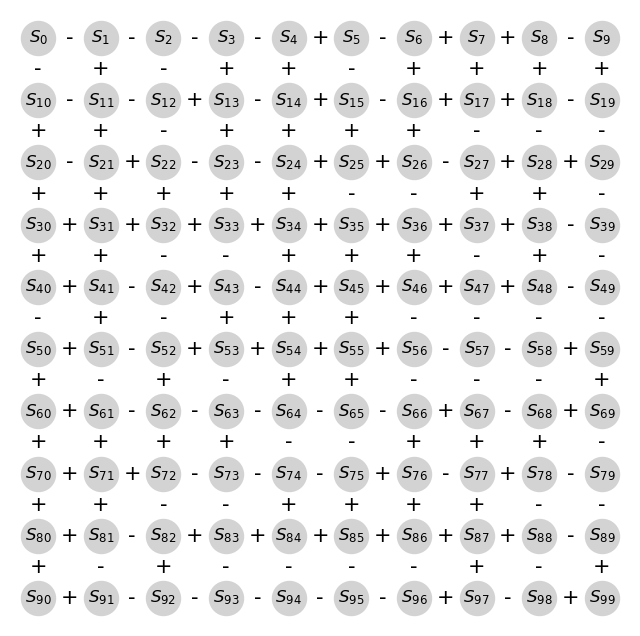
\includegraphics[width=200px]{EA_model}
			\caption {Пример решетки спинов Изинга со случайным распределением обменных констант.}
			\label{fig1}
		\end{center}
	\end{figure}
	
	\section{Модель Изинга}
	Простое математическое описание модели Изинга вместе с отсутствием её точного решения делает её эталоном в теории сложности, так как любая NP-сложная задача может быть сведена к задаче нахождения вектора состояний для модели Изинга со случайным распределением обменных констант~\cite{Markovich2019, papadimitriou1977euclidean, karp2010reducibility}.
	
	В работе энергия взаимодействия спинов Изинга рассчитывается по формуле
	
	\begin{equation}
		E = -\sum\limits_{<i,j>} J_{ij} S_i S_j,
	\end{equation}
	где $S_i, S_j = \pm 1$ - значения спинов, $J_{ij} = \pm 1$ - константа обмена между взаимодействующими спинами в модели Эдвардса\,--\,Андерсона, $\left\langle i,j \right\rangle$ - суммирование по ближайшим соседям. Расчёт энергии можно распараллелить, считая по отдельности энергии взаимодействия цепочек спинов, а затем отдельно добавляя взаимодействия между спинами отдельных цепочек. Такой метод распараллеливания удобен и для пересчёта спинового избытка.
	
	\section{Математический подход}
	
	\textbf{Что такое статистическая сумма и почему она важна?}
	
	\textbf{Что такое h?}
	
	
	Рассмотрим одномерную цепочку из трёх спинов. Обозначим $\beta = \frac{1}{kT}$. Примем обменные интегралы $J$ везде равными единице. Статистическая сумма принимает вид:
	
	\begin{equation}
		Z_3 = e^{3\beta - 3\beta h} + 3e^{\beta - h - \beta} + 3e^{\beta h - \beta} + e^{3\beta + 3\beta h}
		\label{eq:stat_3}
	\end{equation}
	
	Присоединим ещё одну цепочку параллельно первой:
	
	\begin{equation}
		\label{eq:stat_3_un}
		\begin{alignedat}{2}
			Z_6 = Z_3 e^{\beta  h-\beta }+Z_3 e^{\beta  h-\beta }+Z_3 e^{\beta  h-\beta }+Z_3 e^{3 \beta +3 \beta  h}+ \\
			Z_3 e^{\beta  (-h)-\beta }+Z_3 e^{\beta  (-h)-\beta }+Z_3 e^{\beta  (-h)-\beta }+Z_3 e^{3 \beta -3 \beta  h}
		\end{alignedat}
	\end{equation}
	
	В результате получаем статистическую сумму для решетки $3 \times 2$:
	
	\begin{equation}
		\label{eq:stat_3_res}
		\begin{alignedat}{2}
			Z_6 = 6 e^{-5 \beta }+12 e^{-\beta }+2 e^{3 \beta }+e^{9 \beta -6 \beta  h}+6 e^{3 \beta -4 \beta  h}+6 e^{-3 \beta -2 \beta  h}+\\
			9 e^{\beta -2 \beta  h}+6 e^{2 \beta  h-3 \beta }+9 e^{\beta +2 \beta  h}+6 e^{3 \beta +4 \beta  h}+e^{9 \beta +6 \beta  h}
		\end{alignedat}
	\end{equation}
	
	В таком присоединении и наращивании решетки и заключается идея представленного алгоритма
	
	\section{Алгоритм}
	На вход алгоритма мы подаем матрицу связей $J$ и линейный размер системы $L$. В результате работы мы хотим получить данные, которые опишут систему во всех ее состояниях, т.е. энергию, спиновый избыток и вырождение состояний.
	
	На первом этапе берутся нулевой и первый столбцы и рассчитывается их плотность состояний как независимых одномерных цепочек и для каждой заполняется четырехмерный массив: первая ось  – это удвоенная максимальная энергия + 1, вторая ось – удвоенный спиновый избыток + 1, третья ось – это конфигурации, ее размер  $2^L$, и четвертая ось имеет размерность количества простых чисел, остатки от деления на которые записываются по этим координатам. Размер этой оси также увеличен на 1 для проверки на совпадение?????. Избежать добавление этой оси можно только в случае размерности системы, не превышающей $8 \times 8$, в ином случае вырождение может выходить за рамки целочисленного встроенного типа данных большинства низкоуровневых языков.
	
	\begin{algorithm}[H]
		\textbf{ВВОД:} Размер решетки и распределение обменных интегралов.\\
		\textbf{ВЫВОД:} Полная плотность состояний.
		\begin{algorithmic}
			\STATE {Создание массива конфигураций одномерной цепочки методом битового сдвига}
			\STATE {Создание G-тензора [конфигурация крайнего слоя][энергия системы][спиновый избыток][набор простых чисел]}
			\FOR {Все слои решетки\\}
			{
				\FOR {Каждая конфигурация внешнего слоя наращиваемой решетки\\}
				{
					\FOR {Каждая конфигурация добавляемой цевочки спинов\\}
					{
						\STATE {Расчёт энергии и спинового избытка}
						\STATE {Атомарное добавление полученного значения вырождения состояния базовой решетки в тензор вырождения получаемой решетки G[конфигурация крайнего слоя][энергия][спиновый избыток][набор простых чисел]}
					}
					\ENDFOR\\
				}
				\ENDFOR
			}
			\ENDFOR
			\STATE{Расшифровка вырождений набора простых чисел}
			\STATE{Переформирование данных из G-тензора в плотность состояний: вырождение, энергия, спиновый избыток}
		\end{algorithmic}
		\caption{Алгоритм расчета плотности состояний методом полного перебора.}
		\label{algo:dos_exhaustive}
	\end{algorithm}
	
	
	
	
	\section{Реализация алгоритма на CUDA}
	Устройство функции представлено в АЛГОРИТМ 1.
	
	Второй этап заключается в соединение двух массивов состояний, полученных на предыдущем шаге, в один новый, размерность которого будет учитывать новое количество спинов.  Реализация функции объединения представлено в АЛГОРИТМ 2.
	
	Третий этап зацикливает первую и вторую функции до конца решетки, формулы для расчета размерности на каждом этапе весьма тривиальны. В последнем приращении у финального массива состояний можно не задавать ось конфигураций.
	
	АЛГОРИТМ 1.
	
	На последнем этапе мы должны раскодировать массив просуммированных остатков от деления на простые числа в массив вырождений, делаем это, основываясь на китайской теореме об остатках и расширенном алгоритме Эвклида~\cite{katz2007mathematics}.
	
	АЛГОРИТМ 2.
	
	При реализации алгоритма с помощью технологии параллельного программирования CUDA ускорение вычислений достигается за счет расчета уникального индекса для каждого CUDA-ядра, что позволяет каждому потоку обрабатывать свой участок данных. Это достигается путем распараллеливания внешнего цикла, где индексы вычисляются как $x = blockIdx.x \times blockDim.x + threadIdx.x$, и итерации по массиву данных с шагом $blockDim.x \times gridDim.x$, что обеспечивает эффективное использование ресурсов GPU и минимизирует время выполнения.
	
	
	
	\section{Реализация алгоритма на OpenMP}
	
	
	
	
	\section{Сравнение быстродействия (расширить описание)}
	В рамках анализа быстродействия алгоритма было проведено сравнение времени работы алгоритма с алгоритмами прямого перебора, написанных на языках программирования Python и С++, с технологиями параллелизации по ядрам процессора (таблица~\ref{Time_Table}). Использование метода прямого перебора для сравнения аргументировано тем, что именно его можно взять за эталон сложности для данных методов. Таким образом, мы смогли наблюдать кратное превосходство разработанного метода, что развивает интерес дальнейших исследований в этой области.
	
	
	\textbf{Добавить описание вычислителей}
	
	
	В таблице~\ref{Time_Table} представлено сравнение времени выполнения авторского алгоритма перебора с классическими алгоритмами перебора с различными реализациями.
	
	\begin{table}[h]
		\begin{center}
			\begin{tabular}{|c|c|c|c|c|c|c|c|c|}
				\hline
				& $4 \times 4$ & $5 \times 5$ & $6 \times 6$ & $7 \times 7$ & $8 \times 8$ & $9 \times 9$ & $10 \times 10$ & $11 \times 11$  \\ \hline
				Один поток Python & 4.09         & -            & ---          & ---          & ---          & ---          & ---          & ---           \\ \hline
				Python + numba    & 0.046        & 66           & ---          & ---          & ---          & ---          & ---          & ---           \\ \hline
				Один поток на C++ & 0.201        & 204.564      & ---          & ---          & ---          & ---          & ---          & ---           \\ \hline
				С++ + OpenMP      & -            & 23.443       & ---          & ---          & ---          & ---          & ---          & ---           \\ \hline
				CUDA              & 0.602        & 2.385        & 15.153       & 89.114          & ---          & ---          & ---          & ---        \\ \hline
			\end{tabular}
		\end{center}
		\caption{Сравнение времени, затрачиваемого на полный перебор систем спинов Изинга в зависимости от реализации алгоритма и размера системы (значения указаны в секундах).}
		\label{Time_Table}
	\end{table}
	
	\section*{Заключение}
	В результате работы алгоритма мы получаем уникальные данные, характеризующие исследуемую систему. Уникальность заключается в том, что можно определить, глобальный ли минимум был найден с помощью алгоритмов, не являющихся точными, например, Монте-Карло или генетического алгоритма~\cite{Panchenko2007}. Также это позволяет определить оптимальное количество шагов для алгоритма Метрополиса, необходимое для нахождения глобального минимума.
	Полученные с помощью алгоритма характеристики состояний позволяют рассчитать свойства спиновых систем, которые без полной плотности состояний получить нельзя. В том числе для классификации решетки Эдвардса\,--\,Андерсона на ферромагнитное, антиферромагнитное состояния, и состояние спинового стекла, а также провести численный эксперимент по определению фазовых свойств таких решеток в поле.
	
	
	
	\begin{thebibliography}{4}
		\setlength{\parsep}{0pt}\setlength{\itemsep}{3pt}
		
		\Bibitem{roma2010ground}
		\by Rom{\'a}, F and Risau-Gusman, S and Ramirez-Pastor, AJ and Nieto, F and Vogel, EE
		\jour Physical Review B—Condensed Matter and Materials Physics
		\paper Ground-state topology of the Edwards-Anderson$\pm$J spin glass model
		\vol 82
		\issue 21
		\pages 214-401
		\yr 2010
		
		\Bibitem{katzgraber2005correlation}
		\by Katzgraber, Helmut G and Lee, Lik Wee
		\jour Physical Review B—Condensed Matter and Materials Physics
		\paper Correlation length of the two-dimensional Ising spin glass with bimodal interactions
		\vol 71
		\issue 13
		\pages 134-404
		\yr 2005
		
		\Bibitem{romero2020high}
		\by Romero, Joshua and Bisson, Mauro and Fatica, Massimiliano and Bernaschi, Massimo
		\jour Computer Physics Communications
		\paper High performance implementations of the 2D Ising model on GPUs
		\vol 256
		\yr 2020
		
		\Bibitem{onsager1944crystal}
		\by Onsager, Lars
		\jour Physical Review
		\paper Crystal statistics. I. A two-dimensional model with an order-disorder transition
		\vol 65
		\pages 117
		\yr 1944
		
		\Bibitem{maren1991logical}
		\by Maren, Alianna J
		\jour Proceedings of the Second Workshop on Neural Networks
		\paper A logical topology of neural networks
		\yr 1991
		
		\Bibitem{grant2020adiabatic}
		\by Grant, Erica K and Humble, Travis S
		\jour Oxford Research Encyclopedia of Physics
		\paper Adiabatic quantum computing and quantum annealing
		\yr 2020
		
		\Bibitem{Korol2021}
		\by Korol, Alyona Olegovna and Captain, Vitaly Yurievich
		\jour Far Eastern Mathematical Journal
		\paper Neural network for determining the Curie temperature of the two-dimensional Ising model
		\vol 21
		\issue 1
		\pages 51-60
		\yr 2021
		
		\Bibitem{janke2008monte}
		\by Janke, Wolfhard
		\jour Computational many-particle physics
		\paper Monte Carlo methods in classical statistical physics
		\pages 79-140
		\yr 2008
		
		\Bibitem{Markovich2019}
		\by Markovich LA
		\jour Information Technology and Systems
		\paper Parallel algorithm based on the Ising model for solving combinatorial optimization problems
		\pages 350--358
		\yr 2019
		
		\Bibitem{papadimitriou1977euclidean}
		\by Papadimitriou, Christos H
		\jour Theoretical computer science
		\paper The Euclidean travelling salesman problem is NP-complete
		\vol 4
		\issue 3
		\pages 237--244
		\yr 1977
		
		\Bibitem{karp2010reducibility}
		\by Karp, Richard M
		\jour Springer
		\paper Reducibility among combinatorial problems
		\yr 2010
		
		\Bibitem{katz2007mathematics}
		\by Katz, Victor J
		\jour Physics Letters A
		\paper The Mathematics of Egypt, Mesopotamia, China, India, and Islam: A Sourcebook
		\yr 2007
		
		\Bibitem{Panchenko2007}
		\by Panchenko, Tatyana Vyacheslavovna and Tarasevich, Yuri Yurievich
		\jour Computational methods and programming
		\paper Comparative analysis of the efficiency of application of genetic algorithms and Metropolis algorithm in problems of solid state physics
		\vol 8
		\pages 77-87
		\yr 2007
		
	\end{thebibliography}
	
	\EndArticle
	
\end{document}
